\documentclass[11pt]{article}
\usepackage[margin=1in]{geometry}                % See geometry.pdf to learn the layout options. There are lots.
\geometry{letterpaper}                   % ... or a4paper or a5paper or ... 
%\geometry{landscape}                % Activate for for rotated page geometry
%\usepackage[parfill]{parskip}    % Activate to begin paragraphs with an empty line rather than an indent
\usepackage{color}
\definecolor{myblue}{rgb}{0.0, 0.0, 0.85}
\usepackage[breaklinks=true, colorlinks=true, linkcolor=red, urlcolor=myblue, citecolor=black]{hyperref}
\urlstyle{rm}
\usepackage{mathptmx}
\usepackage{graphicx}
\usepackage{amssymb}
\usepackage{epstopdf}
\usepackage{sidecap}
\usepackage{authblk}
\usepackage{booktabs}
\usepackage[font=small,labelfont=bf]{caption}
\usepackage{enumitem}
\usepackage{wrapfig}
\usepackage{draftwatermark}
\SetWatermarkText{DRAFT}
\SetWatermarkScale{1.2}
\SetWatermarkColor[gray]{0.85}
\DeclareGraphicsRule{.tif}{png}{.png}{`convert #1 `dirname #1`/`basename #1 .tif`.png}
\pagestyle{plain}

\def\bfr{\bf\color{red}}
\def\bfp{\color{magenta}}
\def\geohub{{\tt geohub}}
\def\resp{respectively}
\def\selah{SELAH}
\def\nch{718}
\def\nh{957\pm94}
\def\dh{10\%\pm9\%}
\def\nce{389}
\def\ne{556\pm83}
\def\de{15\%\pm12\%}

\begin{document}
%\maketitle

\begin{center}
	\Large\bf Highland Park and Eagle Rock's Unsheltered Population Is \\ Unchanged from 2020\\
	\vspace{1ex}
	{\normalsize\rm Louis Abramson, PhD, and Brian Kohan\\ \today 
	}{\bfr \texttt{ -- NOT FOR DISTRIBUTION}}
\end{center}

\noindent {\bf Summary:} Volunteers surveying Highland Park and Eagle Rock (HPER) on 29 April 2021 
identified a total of $310\pm53$ adults experiencing unsheltered homelessness---a non-significant change of
$-5\%\pm16\%$ compared to the 2020 LAHSA Count (90\% CI). Declines of 20\% and 65\%, \resp, in the 
number of rough sleepers and vans were offset by an 87\% increase in tents and makeshift dwellings 
(Figure \ref{fig:rawCounts}). This near-doubling of the most visually salient part of unsheltered 
living would support subjective impressions that the state of homelessness worsened despite the 
total population remaining statistically unchanged. Data from the Coordinated Entry System will 
reveal how changes in sheltered homelessness affected HPER's total unhoused population.
%As COVID-related contractions in health, sanitation, and social 
%services, have deteriorated conditions on the street, such impressions may yet be accurate. 

\begin{table*}[h]
\caption{Unsheltered Data for Eagle Rock/Highland Park}
\resizebox{\linewidth}{!}{%
\begin{tabular}{lccccccccc}
\toprule
 & Persons & Car & Van & RV & Tent & Makeshift & {\bf 2021 Total} & {\bf 2020 Total} & {\bf \% change*} \\
\cmidrule{1-10}
%Eagle Rock & & & & & & & 127 & 105 & $+21\%$\\
%\cmidrule{8-10}
%Highland Park & & & & & & & 177 & 231 & $-23\%$\\
%\cmidrule{8-10}
Counts & 61 & 18 & 18 & 55 & 41 & 30 & {\bf 223} & {\bf 226} & {\bf 1\%} \\
Inhabitants & 61 (16) & 29 (10) & 32 (11) & 79 (15) & 60 (14) & 51 (13) & {\bf 310 (53)} & {\bf 326} & {$\bf-5\%$ \bf(16\%)} \\
Category share & 20\% (5\%) & 9\% (3\%) & 10\% (3\%) & 25\% (5\%) & 19\% (4\%) & 16\% (4\%) & -- & -- & -- \\ \bottomrule
\end{tabular}
}
\caption*{*Neither the change in raw counts nor inferred population is statistically significant 
(parentheses denote 90\% uncertainties). No minors or families were sighted; two transition aged youth
are tallied as ``Persons,'' above.}
\label{tbl:summary}
\end{table*}

%HP: 167 vs. 209
%ER: 142 vs. 117

\begin{figure*}[h]
	\centering
	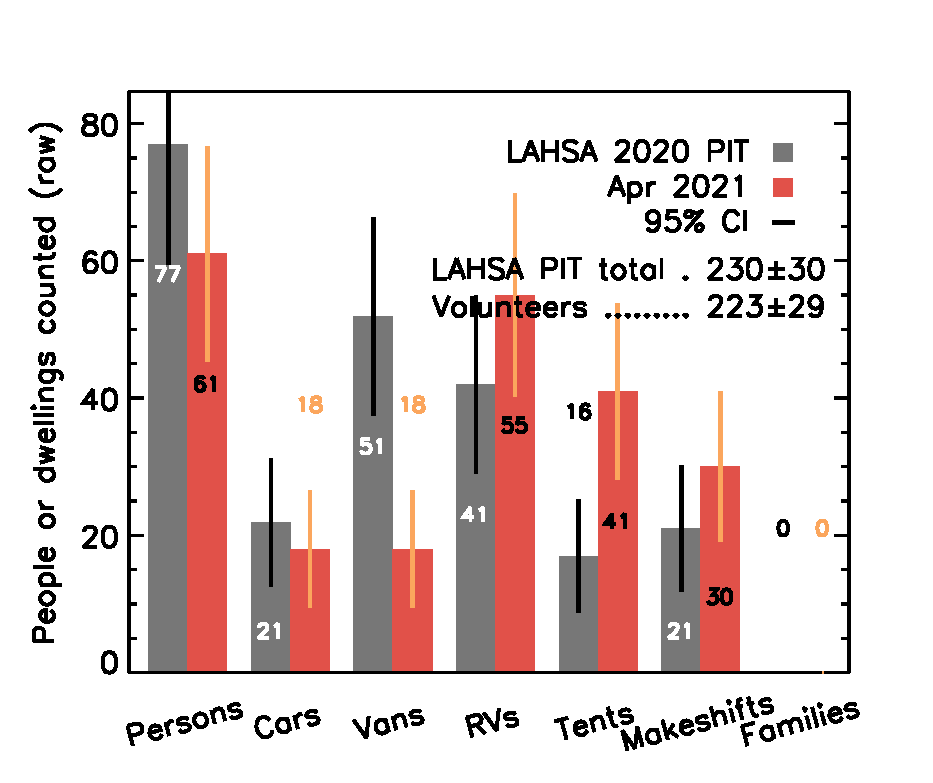
\includegraphics[width = 0.47\textwidth, trim = 1cm 0cm 0cm 1cm]{bars}
	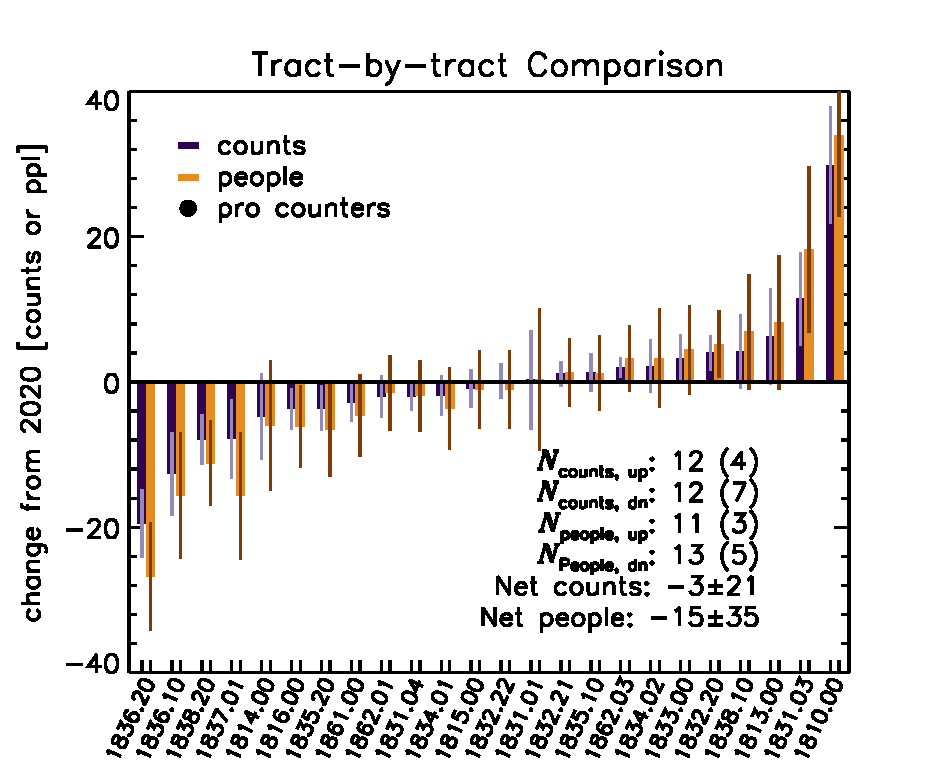
\includegraphics[width = 0.47\textwidth, trim = 0cm 0cm 1cm 1cm]{tractsYrYr.eps}	
	\caption{{\it Left:} total tallies of unsheltered persons + dwellings in Eagle Rock and
			Highland Park from the 2020 and 2021 PIT counts (grey/red). Persons and vans 
			fell while RVs, tents, and makeshift structures rose. Overall, roughly the same number 
			of people + dwellings were identified as in 2020. {\it Right:} tract-level
			results (see also Figure \ref{fig:tcomp}, Table \ref{tbl:allTracts}). Three tracts added 
			significantly more unsheltered people, 5 lost them (parentheses
			denote significant changes). Tract 1836.20 at York/Figueroa saw the largest 
			drop ($-27$ people); 1810.00 along US 134 saw the largest gain ($+34$).}
			%``Persons'' are TAY+Adults.
	\label{fig:rawCounts}
\end{figure*}

%\pagebreak

\noindent {\bf Context:} To compensate for the 
\href{https://laist.com/latest/post/20201209/LAHSA-cancels-2021-homeless-count-los-angeles-covid-19}
{cancellation} of the annual LAHSA Count, volunteers in Highland Park and Eagle 
Rock\footnote{{\bfr ERNC, HHPNC, who else?}} conducted a grassroots vehicle-based enumeration of people 
experiencing unsheltered homelessness in those communities' 24 census tracts on April 29, 2021 
(Figure \ref{fig:tcomp}, top).\begin{wrapfigure}{r}{0.6\linewidth}
	\centering
	\includegraphics[width=\linewidth, trim = -0.5cm 2cm 0.5cm 2cm]{map}
	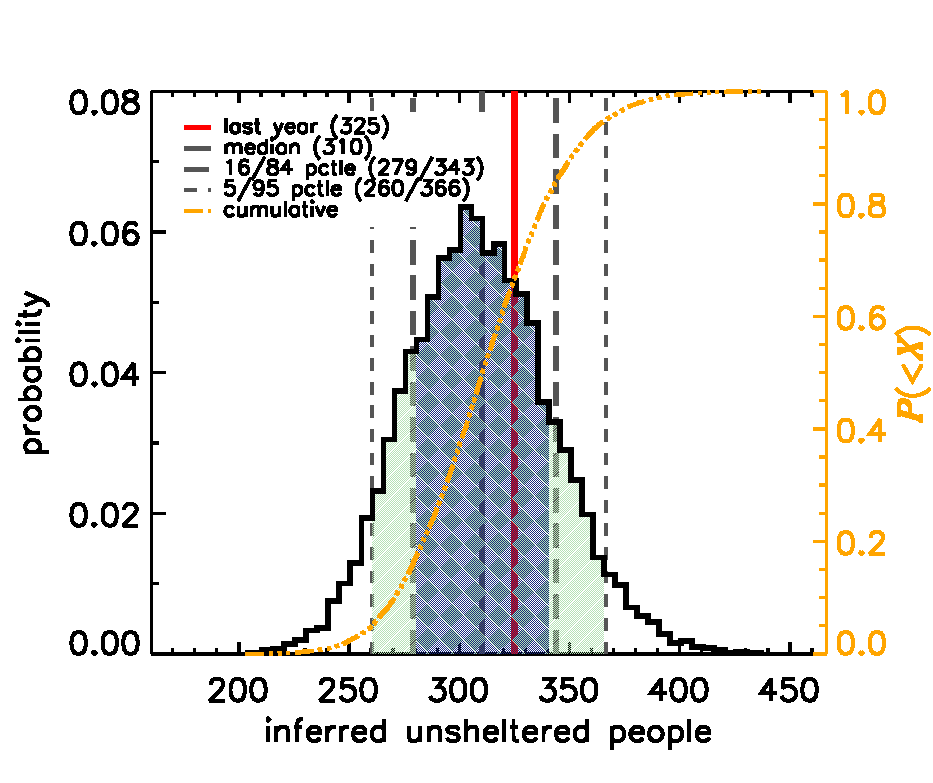
\includegraphics[width=\linewidth, trim = 0cm 0cm 0cm 0cm]{hper2021Hist}
	\caption{{\it Top:} count area with census tracts colored by  
			changes in unsheltered population from 2020 (red$+$, blue$-$).
			Tracts 1836.20 ($-28$ people) and 1810.00 ($+34$) saw the largest swings. 
			{\it Bottom:} the probability distribution for HPER's total unsheltered 
			population. The median is 5\% below 2020's value, but this change is not 
			statistically significant.
			Explore more at \href{https://pit.demoply.org}{pit.demoply.org}.}
	\label{fig:tcomp}
\end{wrapfigure} Surveying ran from 7:00 PM to 11:00 PM.\\

\noindent {\bf Results:} The population estimates in Tables \ref{tbl:summary}, \ref{tbl:allTracts} 
reflect all identified persons, cars, vans, RVs, tents, and makeshift structures with each
dwelling weighted by its average occupancy. We assumed the 
\href{https://www.lahsa.org/documents?id=4635-usc-2018-2020-multipliers-and-estimates-overview}
{SPA4/CD14 weights} adopted in the last official 
\href{https://www.lahsa.org/documents?id=4686-2020-greater-los-angeles-city-community-homelessness-report-service-planning-area-4.pdf}{LAHSA Community Summaries}. Results are unchanged if 
\href{https://www.lahsa.org/documents?id=4693-2020-greater-los-angeles-homeless-count-cvrtm-conversion-factors}{SPA4-wide} occupancies are used instead, or if the tent weight is 
updated based on a survey performed by \href{https://www.selahnhc.org/selah-eagle-rock-chapter}
{SELAH}.\footnote{Outreach teams found 23 people occupying 24 tents in Eagle Rock, yielding an 
estimated $0.96\pm 0.20$ people per tent vs.~LAHSA's 2020 value of $1.48\pm0.11$. Updating the tent 
weight accordingly implies a total HPER unsheltered population of $296\pm49$ people. The implied 
2021 occupancy rises to $1.35\pm0.20$ if 7 tents found to be used for storage are excluded---consistent 
with LAHSA's value, which neglects unoccupied tents.}
% ($296\pm44$ total people) for both SPA4 and using the updated tent weight.

\textbf{Using Monte Carlo methods, we infer HPER's total unsheltered population to be 
310 people---16 people lower than 2020's value. However, counting and weighting uncertainties lead
to a 90\% confidence interval of $\mathbf{\pm53}$ people (Figure \ref{fig:tcomp}, bottom). The 
inferred 5\% decrease is therefore consistent with HPER's \emph{true} unsheltered population 
remaining the same as it was last year.}

At the community level, Highland Park's 17 tracts saw a 23\% drop ($183\pm41$ vs.~220 people
last year; 92\% chance of decline); Eagle Rock's 7 tracts saw a 21\% rise ($127\pm28$ vs.~105; 92\% 
chance of increase). The latter is attributable to tract 1810.00, wherein new encampments have arisen 
along US 134. If that tract is excluded, Eagle Rock's unsheltered population 
remained statistically stable ($68\pm22$ people vs.~79 in 2020).

%, such that 22/100 simulated surveys would have found \emph{fewer} unsheltered people compared to last year

%\begin{wrapfigure}{l}{0.625\linewidth}
%	\centering
%	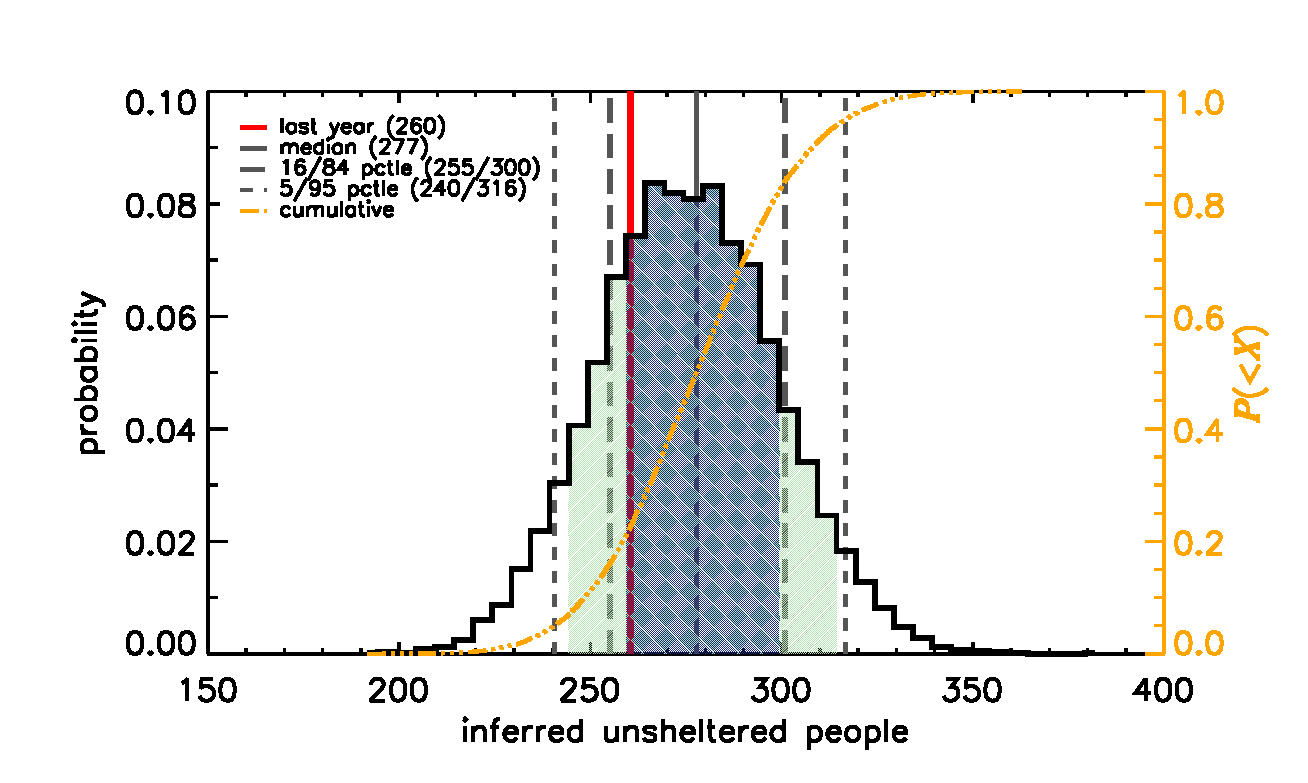
\includegraphics[width=\linewidth, trim = 0cm 0cm 0cm 0cm]{mcw2021Hist}
%	\caption{Probability distributions for the total unsheltered population in Mid City West.}
%	\label{fig:hist}
%\end{wrapfigure} 

Each of the 24 total tracts were counted once, with parkland areas in two tracts surveyed on foot
earlier in the day (Table \ref{tbl:allTracts}). In two additional tracts, only the ``b'' splits were counted
to conform the survey to HPER borders as defined by LAHSA and the 
\href{https://statisticalatlas.com/neighborhood/California/Los-Angeles/Eagle-Rock/Overview}{Statistical Atlas}. 
Splits 1851.00c and 
1994.00a---which LAHSA may affiliate with ``Highland Park'' and which contained 37 unsheltered 
people in 2020---were also not counted. The count uncertainty is $\pm$13\% (95\% CI), 
with the remainder of the $\pm$17\% total population margin of error due to ranges in 
dwelling occupancies.\\

\begin{wraptable}{r}{0.50\linewidth}
\caption{Tract-level Unsheltered Populations}
\resizebox{\linewidth}{!}{%
\begin{tabular}{cccc}
\toprule
Tract & Passes & Unshelt pop. & 90\% CI \\ 
\cmidrule{1-4}
1810.00$^{\rm a}$  & 1 & 59 & 44--74 \\
1813.00  & 1 & 33 & 22--45 \\
1814.00  & 1 & 21 & 10--31 \\
1815.00  & 1 & 4 & 0--11 \\
1816.00$^{\rm a}$  & 1 & 2 & 0--9 \\
1831.01  & 1 & 31 & 19--43 \\
1831.03  & 1 & 40 & 25--58 \\
1831.04  & 1 & 1 & 0--8 \\
1832.20  & 1 & 6 & 0--13 \\
1832.21  & 1 & 3 & 0--10 \\
1832.22  & 1 & 4 & 0--11 \\
1833.00  & 1 & 11 & 1--19 \\
1834.01  & 1 & 4 & 0--11 \\
1834.02  & 1 & 12 & 3--22 \\
1835.10  & 1 & 6 & 0--13 \\
1835.20  & 1 & 5 & 0--13 \\
1836.10  & 1 & 15 & 5--24 \\
1836.20  & 1 & 1 & 0--8 \\
1837.01  & 1 & 15 & 6--23 \\
1838.10  & 1 & 22 & 11--32 \\
1838.20  & 1 & 3 & 0--10 \\
1861.00$^{\rm b}$  & 1 & 3 & 0--10 \\
1862.01  & 1 & 4 & 0--11 \\
1862.03$^{\rm b}$  & 1 & 3 & 0--10 \\
\cmidrule{1-4}
{\bf All} &{\bf 24} & {\bf 310} & {\bf 250--366}
\\ \bottomrule
\end{tabular}
}
\caption*{$^{\rm a}$ Rec center surveyed on foot circa 3:00 PM; $^{\rm b}$ Split ``b'' only.}
\label{tbl:allTracts}
\end{wraptable}

\noindent {\bf Comments:} The above results reflect a {\bf 20\% drop in adult individuals} 
 seen on the street---mirroring trends in 
\href{https://www.latimes.com/homeless-housing/story/2021-04-13/despite-appearances-15-fewer-homeless-people-were-on-hollywood-streets-this-year}{Hollywood} and Mid City West---a {\bf 65\% 
drop in identified van dwellings}, and an {\bf 87\% increase in tents and makeshift structures}. 
While the decline in vans is too large to reflect the 10--20 Safe Parking spots in neighboring
Glassell Park, government initiatives to stop evictions and move people off the street may have 
done enough additional work to hold the total population stable. 
If \href{https://www.lahsa.org/documents?id=4673-2020-homeless-count-council-district-14}{CD14's} 11\% share of \href{https://www.lahsa.org/documents?id=4585-2020-greater-los-angeles-homeless-count-los-angeles-continuum-of-care-coc-}{LA County's unsheltered seniors} 
is an indication, 200 CD14 residents might have been in any of Project Roomkey's 
\href{https://projectroomkeytracker.com/}{1,826 active rooms} on the night of the 
count.\footnote{Due to the presence of Skid Row, CD14-level trends may not
reflect those in HPER.} {\bfr Other known shelters?} Coordinated Entry System data will show 
if the above scenarios are true.

While the number of people on the street may be unchanged, their quality of life has worsened. 
COVID has restricted or eliminated access to restaurant bathrooms, libraries 
(\href{https://www.lapl.org/homeless-resources/the-source}{\it The Source}), DPSS 
(EBT, Medi-Cal), DMV (IDs), and DMH facilities. Physical limits on client access at 
hospitals has also kept caseworkers from managing successful discharges. These harms 
are reflected by a 33\% increase in 
\href{http://publichealth.lacounty.gov/chie/reports/HomelessMortality2020_CHIEBrief_Final.pdf}{overdose deaths} and made more visible by \href{https://clkrep.lacity.org/onlinedocs/2020/20-0147_misc_3-17-20_p.pdf}{suspended}
tent folding and sanitation practices as tents increased.
Of course, with no significant decline observed with them in place, a substantial rise in unsheltered 
homelessness is likely \href{https://www.latimes.com/california/story/2021-01-12/new-report-foresees-tens-of-thousands-losing-homes-by-2023}
{once the eviction moratoria lapse}.

The data support the effectiveness of programs aimed at curbing a rise in street homelessness.
Yet, they do {\it not} suggest that the state of homelessness has improved. In the fight to rebuild 
lives as we build homes, that fact must remain paramount.

%\clearpage

\end{document}  